% -*- mode: latex-mode; TeX-engine: xetex; LaTeX-command-style: (("" "SOURCE_DATE_EPOCH=0 %(PDF)%(latex) --shell-escape %S%(PDFout)")); TeX-master: "../dissertation.tex"; -*-

\chapter{Computer Control of the Experiment}
\label{ch:computer-control}

\section{Introduction}

The experiment sequence and data taking is managed by computers.
In additional to controlling the timing and the actions during a sequence,
the computer control system is also the main interface
between the people running the experiment (the user),
the data and the hardware performing the manipulation and measurements.
Because of its central role in the experiment,
it has to satisfy many requirements so that
the daily operation of the lab can be performed smoothly and reliably.
\begin{enumerate}
\item Full control and utilization of hardware.\\
  The control system is a layer in between the the user and the hardware
  and will abstract and manage the hardware on behave of the user.
  However, the abstraction must still allow the user to take advantage of
  the full capability of the hardware, e.g. output resolution, timing accuracy etc..
  This is because there is usually little margin between the capability of the hardware
  and the requirement in the experiment as the specification of the hardware
  is often selected based on the requirement to begin with.
\item Usability for all lab members.\\
  The lab is operated by users with specialty in physics rather than computer science.
  Although some basic knowledge of computer programming is required for operating
  the experiment as well as analysing data,
  the computer control system must be fully usable for people without any experience
  in building complex software systems.\\
  The inevitable complexity of the system must be fully hidden from the user
  for normal operations although more direct control may still be allowed in certain cases.
\item Modeling of the sequence and scan.\\
  As an important special case of usability,
  the computer control system must provide a model for each tasks closed to
  the users' mental model.
  More concretely, this means creating abstraction for concepts
  typically used to describe the task and allow operation on these abstractions
  matching the users' expectation.
  We will talk about concrete examples of this requirements
  in section \ref{ch:computer-control:frontend} regarding the sequence frontend
  and section \ref{ch:computer-control:scan} regarding scan automation.
\item Reproducibility.\\
  When exploring something new in the experiment,
  trial and error is the standard method and troubleshooting is a major part of the process.
  The ability to do this effectively requires a high degree of reproducibility of all the result.
  While it is impossible and also not the job of the computer control system to
  eliminate all the fluctuation and noise in the experiment,
  it should not add to the randomness of the system.
  With few exceptions, identical user input should produce identical output from
  the control system.
\item Version control.\\
  As a variation of the reproducibility requirement and also built on top of it,
  we must be able to revert to a previous software configuration at a later time
  in order to reproduce and double-check an earlier result.
  The use of a proper version control system on the settings and code for
  the computer control system can allow this with additional features
  including easy visualization of setting change and parallel development of code
  by multiple users.
\end{enumerate}

The design of the computer control system is mainly guided by these requirements
and we will go into more detail as we describe each part of the system.
The application programming interface (API) provided for sequence and scan programming
are mostly text based due to the flexibility and version control requirement.
Some graphic user interface (GUI) are also included for specific tasks
built on top of the text interface but will not be covered in this chapter.
Section \ref{ch:computer-control:frontend} will cover the frontend of the system
which is used by the user directly to specify an experimental sequence.
Section \ref{ch:computer-control:backend} will discuss the support for various
hardware backends used to run a sequence.
After that, section \ref{ch:computer-control:scan} describes how multiple sequences
can be put together to form a scan and
we will talk about some planned update to the system in section
\ref{ch:computer-control:summary}.

\section{Frontend}
\label{ch:computer-control:frontend}

The frontend is the main user interface of the system to specify a sequence.
Its API is designed around the a few concepts that can be divided into two categories,
\begin{enumerate}
\item Timing
  \begin{enumerate}
  \item (Sub-)sequence\\
    This represent a series of events that has fixed relative timing.
    Sequences can be nested in other sequences at a specific time offset
    and are called subsequences.
    Each sequence can only have at most one parent sequence (the top level one has none)
    and zero or more subsequences so all the subsequences in a top level sequence forms a tree.
  \item Time step\\
    The time or time period in the sequence when one or more event may happen
    is called a time step.
    Each time step has a length and a position within a unique parent sequence
    and are always the leaves on the sequence tree.
  \end{enumerate}
\item Output
  \begin{enumerate}
  \item Channel\\
    Each device that can generate an output are abstracted into
    one or multiple channels that each output a single number.
    The abstraction depends on the type of the device,
    e.g. voltage value for a digital to analog converter,
    or frequency and amplitude for an computer-controlled sine-wave generator.
  \item Pulse\\
    This represents the actual output for a particular channel.
    The pulse itself does not contain the timing information within the sequence,
    i.e. start and end time.
    Instead, each pulse belongs to a unique time step that specifies the timing.
  \end{enumerate}
\end{enumerate}
Operations on concepts in one category are usually independent of the other
which allows most common modifications to the sequence to be done
with minimum code change, including,
\begin{enumerate}
\item Adding/removing/changing the length of time step or subsequences
  without affecting the relative timing or output in other part of the sequence.
\item Enabling/disabling output or changing output values
  without changing the time and length of the output.
\end{enumerate}

The sequence programming uses MATLAB as the host language.
Despite not the best choice from the feature or performance aspect,
it offers the following desired properties,
\begin{enumerate}
\item Text based language and therefore easier for version control.
\item Familiarity for physics student.\\
  MATLAB is often used for simulation and data processing.
  It is one of the few languages that most new students will be familiar with.
\item Builtin feature-rich integrated development environment (IDE).
\item Foreign function interface (FFI).\\
  Other parts of the system needs to be implemented in other languages
  for various reasons including higher performance.
  It is important that we can call into other languages to allow such a hybrid implementation.
\item Good enough feature set.\\
  MATLAB provides data structures like arrays and hash table
  as well as handle classes with object identity
  which are important to handle the representation of the sequence.
  It also has an good enough object-oriented programming (OOP) model
  and operator overloads which can simplify the API syntax for the user.
\end{enumerate}

\subsection{Channel Naming}
Each output channel has a unique name attached for identification.
This name is always a string of the format \verb`<device_id>/<channel>`
where \verb`<device_id>` is an name for the (physical) device
and \verb`<channel>` is an identification of the channel within the device.
The \verb`<device_id>` may not contain \verb`/` but other than this
neither \verb`<device_id>` nor \verb`<channel>` has globally predefined meaning
and are completely up to the backend to define.
This format allows maximum freedom for the backend to abstract its function
into multiple channels in the most fitting way,
while allowing the generic code to identify the device, and therefore backend,
needed without fully interpreting the channel name.

\subsection{APIs}
\begin{figure}
  \centering
  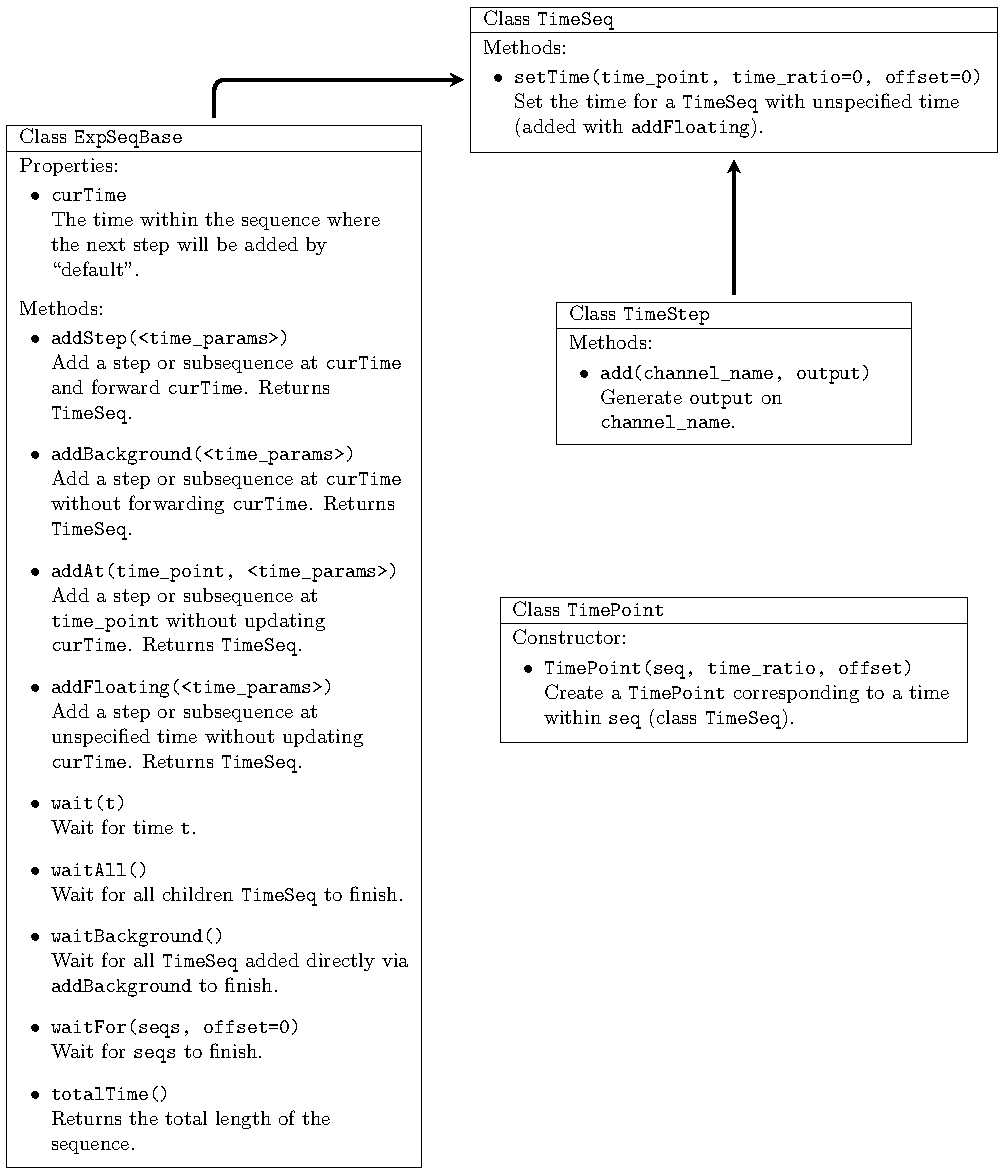
\includegraphics[width=\textwidth]{figures/computer_control_frontend_classes.pdf}
  \caption[Frontend API classes]{
    Frontend class inherit diagram and API lists.
    \label{fig:computer-control:frontend-classes}}
\end{figure}

The system provides the following APIs for sequence creation
that are subject to strict backward compatibility requirements.
The most important APIs are listed in this section.
Fig.~\ref{fig:computer-control:frontend-classes}
provides a short summary of all the classes and methods mentioned in this section.

\subsubsection{Timing}
Subsequences are represented by the \verb`ExpSeqBase` class
and time steps are represented by the \verb`TimeStep` class.
Both \verb`ExpSeqBase` and \verb`TimeStep` are subclasses of \verb`TimeSeq`,
which represent an arbitrary node on the sequence tree.

Most timing related APIs are methods on \verb`ExpSeqBase`.
The most important ones are the ones creating new branches
in the subsequence tree, i.e. \verb`TimeSeq`.
The type of the branch created is determined by the parameters passed in
(\verb`<time_params>`), which can be either,
\begin{enumerate}
\item \verb`length, offset=0`\\
  This creates a new \verb`TimeStep` with a numerical \verb`length`
  and an optional time \verb`offset` from a API dependent time reference point
  (see list of APIs below).
\item \verb`offset=0, callback, <callback parameters>`\\
  This creates a new \verb`ExpSeqBase` with an optional time \verb`offset`
  the time reference point.
  The new subsequence will be populated by calling \verb`callback`
  with the new sequence followed by \verb`<callback parameters>`.
\end{enumerate}
Since most sequences are built in series, \verb`ExpSeqBase` maintains
a current time (\verb`curTime`) of the sequence.
Various methods are provided that acts differently with respect to \verb`curTime`.
\begin{enumerate}
\item \verb`addStep(<time_params>)` method\\
  This is the most used method to construct the sequence in series.
  The time reference point is \verb`curTime` and
  \verb`curTime` will be set to the end of the time step or subsequence created.
  A check is make sure the \verb`curTime` only moves forward and
  errors if a too negative \verb`offset` is specified.
  This ensures that what added with \verb`addStep` always appears in the final
  sequence in the same order as program execution order
  which makes the code easier to reason about.
\item \verb`addBackground(<time_params>)` method\\
  The time reference point is \verb`curTime` and no change to \verb`curTime` is made.
\item \verb`addAt(time_point, <time_params>)` method\\
  The time reference point is specified by \verb`time_point` which is of type \verb`TimePoint`.
  See below about \verb`TimePoint`.
\item \verb`addFloating(<time_params>)` method\\
  The time reference point is unspecified.
  The optional \verb`offset` parameter cannot be specified in \verb`<time_params>`.
  The time reference point, however, must be specified before the sequence can run.
  This can be done by calling the \verb`setTime(time_point, time_ratio=0, offset=0)` method
  on the \verb`TimeSeq` object returned,
  where \verb`time_point` is also of type of type \verb`TimePoint` described below.
  The optional \verb`time_ratio` specifies the relative time within the subsequence
  or time step to set the time for where a value of $0$ set the start time
  and a value of $1$ set the end time.
\end{enumerate}
All methods return the new \verb`TimeSeq` constructed so that they can be operated on.

The \verb`TimePoint` object used in \verb`addAt` and \verb`setTime`
can be constructed via \verb`TimePoint(seq, time_ratio, offset)`
which represent the time within the sequence or step \verb`seq` with a time \verb`offset`.
\verb`time_ratio` specifies the time within the \verb`seq` where $0$ is the start time
and $1$ is the end time.

Additional continence methods for \verb`ExpSeqBase` are also provided
to manipulate \verb`curTime`,
\begin{enumerate}
\item \verb`wait(t)` method\\
  Add \verb`t` to \verb`curTime`.
  This is the only method that can change \verb`curTime` backwards.
\item \verb`waitAll()` method\\
  Forward \verb`curTime` to the end of all (nested) subsequences and time steps
  within the current subsequence.
\item \verb`waitBackground()` method\\
  Similar to \verb`waitAll()` but only wait for the subsequences and time steps
  directly added to the current subsequence.
\item \verb`waitFor(seqs, offset=0)` method\\
  Forward \verb`curTime` to the end of subsequences and time steps specified
  within the array \verb`seqs`.
  An optional \verb`offset` may be added to the latest end time.
\end{enumerate}

\subsubsection{Output}

As mentioned before, all the output are specified on time steps
which are represented by class \verb`TimeStep`.
This is done via a single method \verb`add(channel_name, output)` on \verb`TimeStep`.
The \verb`channel_name` is the channel name described above
and \verb`output` specifies the output in one of the following way,
\begin{enumerate}
\item A number\\
  This represent setting the channel to the specified value at the start time of the pulse.
\item A function or callable object\\
  The function will be used to compute the value to output over the whole duration of the pulse.
  It will be called with arguments \verb`(t, len, old_val)` where
  \verb`t` is the time within the pulse, \verb`len` is the length of the pulse
  and \verb`old_val` is the previous value of the channel before the current pulse.
\end{enumerate}

\section{Backends}
\label{ch:computer-control:backend}
As discussed in section \ref{ch:computer-control:frontend},
the frontend provides an API to program all the output channels in the same way
no matter the type of the channel or device used.
However, this is not the case for the devices generating for the output
which often have an API specifically designed for the device
that may be very different from one another.
Moreover, the frontend represent the sequence as a tree structure
that is convinient for manipulation
whereas the device API typically uses a flat data structure like an array of numbers
or a series of commands.
It is therefore the job of the backend to bridge this gap
and convert the between the multiple representations of the sequence.
The conversion is done in a ``generate'' step and
the result is cached for each sequence to allow running the sequence
multiple times with minimum overhead.

The specific requirements and implementations for each backends are very different.
Nevertheless, there are a few important features or components that are shared among
different backends.

\subsection{Network Communication}
\label{ch:computer-control:backend:net}
With one current exception, the output device is not directly connected to
the computer running the frontend but is only connected to another computer
on the same network.
This requires network communication between the frontend machine and
a service running on the device computer for running the sequence.

We use ZeroMQ Message Transport Protocol (ZMTP) as the main protocol for network communication
which offers the following advantages,
\begin{enumerate}
\item Binary protocol\\
  The protocol allows us to send and recieve arbitrary data without having to encode it
  in text first. This saves encoding and decoding time as well as network bandwidth
  which allows higher performance.
\item Feature rich and flexible\\
  Compared to using sockets for network communication directly,
  the message oriented protocol allows easy implementation of remote procedure call (RPC).
  The ZeroMQ library also provides flexible interface to process the messages
  which is useful to implement robust handling of failure
  and parallel processing of requests.
\item Light weight\\
  Despite the rich feature set, the library is relatively light weight.
  This is important because part of the computer control system
  need to be executed in environment with limited resources.
\item Cross platform\\
  The library is cross platform and provide identical API on different environment.
  Windows support is particularly important since most of the development is done
  on Linux machines.
\item Stable\\
  Both the protocol and the library are stable.
  The library version available on different machines are not always the same
  and it is important that the same version of code can work on different machines
  and can communicate with each other in all cases.
\end{enumerate}

\subsection{Sorting of Pulses}
The tree representation of the sequence is useful for construction and manipulation
but contains unnecessary information for generating output,
for which only the pulses and their start and end time
within the top-level sequence is important but not the subsequence structure.
Because of this, all the backends starts the generation step by
flattening the tree to obtain a list of all pulses sorted by their start time.
After the sorting of the pulses, the tree structure is discarded by default
\footnote{This behavior can be disabled for debugging purpose} to reduce memory usage.

\subsection{Representation of Pulses}
Several backends require accessing the exact representation of the pulses
outside MATLAB code and even on a different computer.
Since the pulses can be arbitrary functions,
this requires the ability to serialize and deserialize code.

In order to do this, we developed a simple intermediate representation (IR)
of code that runs on a register-based virtual machine.
The IR supports three different data types, \verb`Bool`, \verb`Int32` and \verb`Float64`
and basic arithmetic, control flow and math functions
that are sufficient for specifying pulse shapes.
The IR can be interpreted by an interpreter written in C++ or
be compiled and optimized to native code for faster execution using an LLVM based compiler.

In order to convert MATLAB functions specified in the sequence to the IR,
we pass in a special object as the input argument to the MATLAB function.
Supported operations on this object will return a new object
that records the operation as well as input arguments.
The value returned from the function is therefore an object representing
all the operations needed to compute the result as a directed acyclic graph (DAG).
We then convert each node in the DAG to an IR instruction to finish the convertion.
This process only support pure functions.
Conditional branch is supported via an \verb`ifelse` function
that returnes one of the input argument based on an condition.
Loops are not currently supported.

\subsection{FPGA Backend}
\begin{figure}
  \centering
  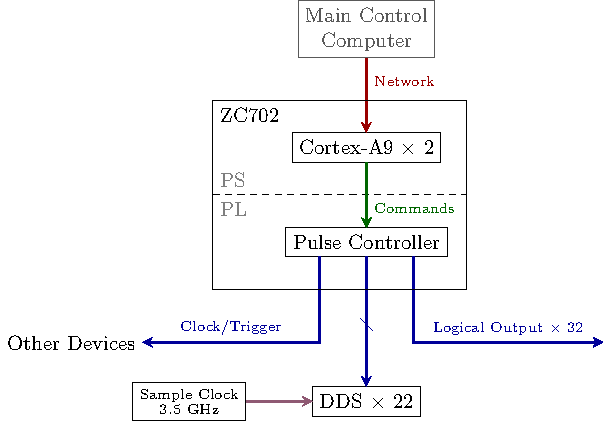
\includegraphics[width=0.9\textwidth]{figures/computer_control_backend_fpga.pdf}
  \caption[FPGA Block Diagram]{
    FPGA hardware block diagram.
    The sequence data is sent to the server program running on the CPU via network.
    The program then push the commands to the pulse controller implemented
    in the programming logics.
    The pulse controller executes the commands and genenerates or changes outputs
    for clock/trigger, DDS or logical outputs.
    \label{fig:computer-control:backend-fpga}}
\end{figure}
The timing of the experiment is controlled by a Xilinx ZC702 FPGA
which contains both a processing system (PS) part, i.e. CPU,
and a programmable logic (PL) part, i.e. FPGA (Fig.~\ref{fig:computer-control:backend-fpga}).
The PL creates digital control signals for various peripheral devices
which generate output for the experiment,
including direct digital synthesizers (DDS), logical switching signal
and clock or trigger signal for other devices.
The PS consists of a dual core Cortex-A9 CPU
which runs an Arch Linux ARMv7 distribution.
The server software that runs on the PS communicates with the main control computer
via ZeroMQ (\ref{ch:computer-control:backend:net})
and generates a custom command stream to control the PL output.
Each command corresponds to making one change to the final output, e.g.
logical values, DDS output amplitude or frequencies, etc.
The main job of the FPGA backend is therefore to convert
the sorted pulses to the command stream.

Due to performance concern, this conversion is done in C++ code\footnote{\url{https://github.com/nacs-lab/libnacs/blob/0076e347ff3ba674fbf74872883b40feefd82ce0/lib/seq/bytecode.cpp\#L528}}.
The main design considerations and features are,
\begin{enumerate}
\item The sequence supports changing and ramping multiple channels at the same time.
  This is not supported by the hardware due to the limit on the number of I/O ports
  connecting the PL to the output devices requiring multiplexing of the control signal.
  The backend manages this by interleaving the commands for different channels
  when more than one are changed at the same time.
  A set of active pulses are maintained as the conversion proceed through sequence time.
  Pulses are added to the active set when the start time is reached
  and retired from the set when the end time is reached.
\item For a continuous ramp of a channel, since the output changes are discrete,
  it may not happen at exactly the end time of the pulse
  which requires special care to ensure the correctness of the channel value after a pulse.
  For example, a linear ramp from $0$ to $0.5$ on a channel from time $0 \mathrm{\mu s}$
  to $5 \mathrm{\mu s}$ may only receive update at time $0, 2, 4 \mathrm{\mu s}$
  with values $0.0, 0.2, 0.4$ respectively due to discretization.
  However, the user should expect the value of the channel (absence of other pulses)
  long after the pulse to be $0.5$ instead.
  This is handled in the backend by checking the last update from the pulse
  against its expected ending value before retiring it.
  A final update to the ending value is generated if the two values are different.
\item The output has finite resolution.
  If an update changes the value that is unresolved by the hardware
  (typical during a slow ramp), the update will be omitted.
\item Some commands correspond to more than one action/pulse in the sequence.
  For example, more than one logical outputs can be updated at the same time
  and some commands also accept a variable wait time afterwards
  (in additional to a special purpose wait command).
  The backend examines neighboring operations and may merge multiple commands into one.
  This is especially useful for logical outputs.
  In fact, logical outputs changes that is specified to happen at the same time in the sequence
  are guaranteed to happen at the same time in the experiment as well.
\item The PL commands are fixed length to allow a simpler implementation
  of command parsing in the PL.
  However, since not all commands contain the same amount of information,
  some include padding for alignment.
  In order to save network bandwidth, a compressed format with variable command length
  and no padding is used to transfer the commands through the network.
  The decompression is done when running the sequence on the CPU right before
  sending to the PL for execution.
\end{enumerate}

\subsection{NiDAQ Backend}
(Variable clock)
% \item (clock generation)

\subsection{USRP Backend}
(SIMD)

\section{Automation of Scans}
\label{ch:computer-control:scan}

(Scan requirement)
(Combination of scans)
(Scope/nested structure)

\section{Summary and Outlook}
\label{ch:computer-control:summary}
(new backend/SPCM)
(native code generation, auto vectorization)
(dynamic logic and dependency tracking/optimization)
